% !TEX encoding = UTF-8
% !TEX program = pdflatex
% !TEX spellcheck = it_IT

\documentclass[a4paper, 11pt]{article}

% sintassi
\usepackage[T1]{fontenc}
\usepackage[utf8]{inputenc}
\usepackage[english]{babel}
\DeclareUnicodeCharacter{00A0}{~}
\usepackage{fullpage}
%\usepackage[cochineal]{newtxmath}
%\usepackage{crimson,verbatim}
\usepackage[charter]{mathdesign}
\usepackage{textcomp}
\usepackage{color,soul,hyperref,mwe}

% matematica e chimica

\usepackage{siunitx,amsmath,bm,chemfig}
\newcommand{\ud}{\mathop{}\!\mathrm{d}}
\sisetup{detect-all,math-rm = \ensuremath}

\setatomsep{2em}

\newcommand\setpolymerdelim[2]{\def\delimleft{#1}\def\delimright{#2}} 
\def\makebraces[#1,#2]#3#4#5{% 
\edef\delimhalfdim{\the\dimexpr(#1+#2)/2}% 
\edef\delimvshift{\the\dimexpr(#1-#2)/2}% 
\chemmove{% 
\node[at=(#4),yshift=(\delimvshift)] {$\left\delimleft\vrule height\delimhalfdim depth\delimhalfdim 
width0pt\right.$};% 
\node[at=(#5),yshift=(\delimvshift)] 
{$\left.\vrule height\delimhalfdim depth\delimhalfdim 
width0pt\right\delimright_{\rlap{$\scriptstyle#3$}}$};}} 
\setpolymerdelim()

% tabelle e grafica
\usepackage{booktabs,graphicx,subfig,caption,pdfpages}
\captionsetup{font=small,
	format=hang,
	justification=centering,
	singlelinecheck=true,
	labelfont={sf,bf}	
}
\usepackage{float}
\floatstyle{plaintop}
\restylefloat{table}
\usepackage{multirow}
\usepackage{fancyhdr}
\pagestyle{fancy}
\fancyhead[LE,RO]{\textsl{\rightmark}}
\fancyhead[LO,RE]{\nouppercase{\leftmark}}
\fancyfoot[C]{\thepage}
\usepackage[margin=1in,headsep=.3in]{geometry}
\usepackage[suftesi]{frontespizio}
\usepackage{xparse}
\setlength\parindent{0pt}

\newenvironment{chapterabstract}{%
  \par\nobreak\noindent
  \textbf{\textit{Abstract}\hrulefill}\nobreak
  %\small
  \noindent\ignorespaces
}{%
  \par\nobreak\normalsize
  \vskip-\ht\strutbox\noindent
  \textbf{\hrulefill}%
}
\makeatletter
\NewDocumentCommand\headerspdf{ O {pages=-} m }{% [options for include pdf]{filename.pdf}
  \includepdf[%
    #1,
    pagecommand={\thispagestyle{fancy}},
    scale=1,
    ]{#2}}
\NewDocumentCommand\secpdf{somO{1}m}{% [short title]{section title}[page specification]{filename.pdf} --- possibly starred
  \clearpage
  \thispagestyle{fancy}%
  \includepdf[%
    pages=#4,
    pagecommand={%
      \IfBooleanTF{#1}{%
        \section*{#3}}{%
        \IfNoValueTF{#2}{%
          \section{#3}}{%
          \section[#2]{#3}}}},
    scale=.65,
    ]%
    {#5}}
\makeatother

\begin{document}



\begin{chapterabstract}



\end{chapterabstract} 

\section{Experimental activity}

\subsection{Injection molding: sample evaluation}
Different speciments of unknown polymeric materials have been analysed and identified. They have been produced by injection molding according to specific standards (ISO and ASTM).
\begin{itemize}
\item ISO 10.0 x 4.0 x 172 (mm);
\item ASTM 12.7 x 3.2 x 165 (mm);
\end{itemize}

Size of all speciments and the mold cavity have been measured through a caliper in order to evalaute the shrinkage after the process.
ASTM samples (with sprue and bar) have been weighted through the balance METTLER PM ${4600}$ in order to compare the total weight and polymer density.

\section{Results and discussion}
\subsection{Injection molding: sample evaluation}

ISO speciments are reported in Figure \ref{fig:ISO}.

\begin{figure}[htp]
\centering
\subfloat[][]
{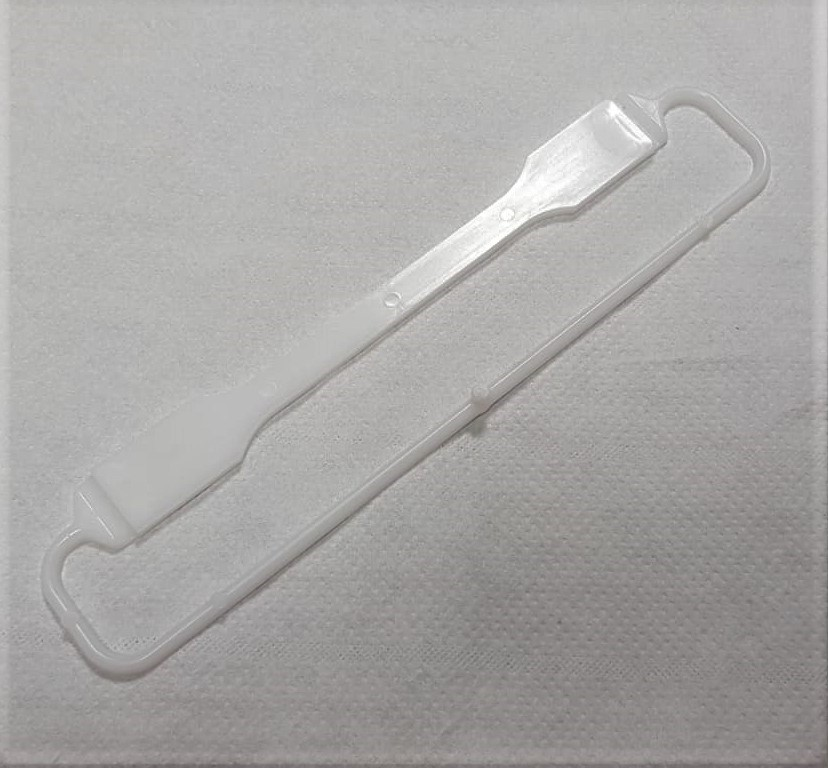
\includegraphics[scale=0.212]{POM}} \qquad
\subfloat[][]
{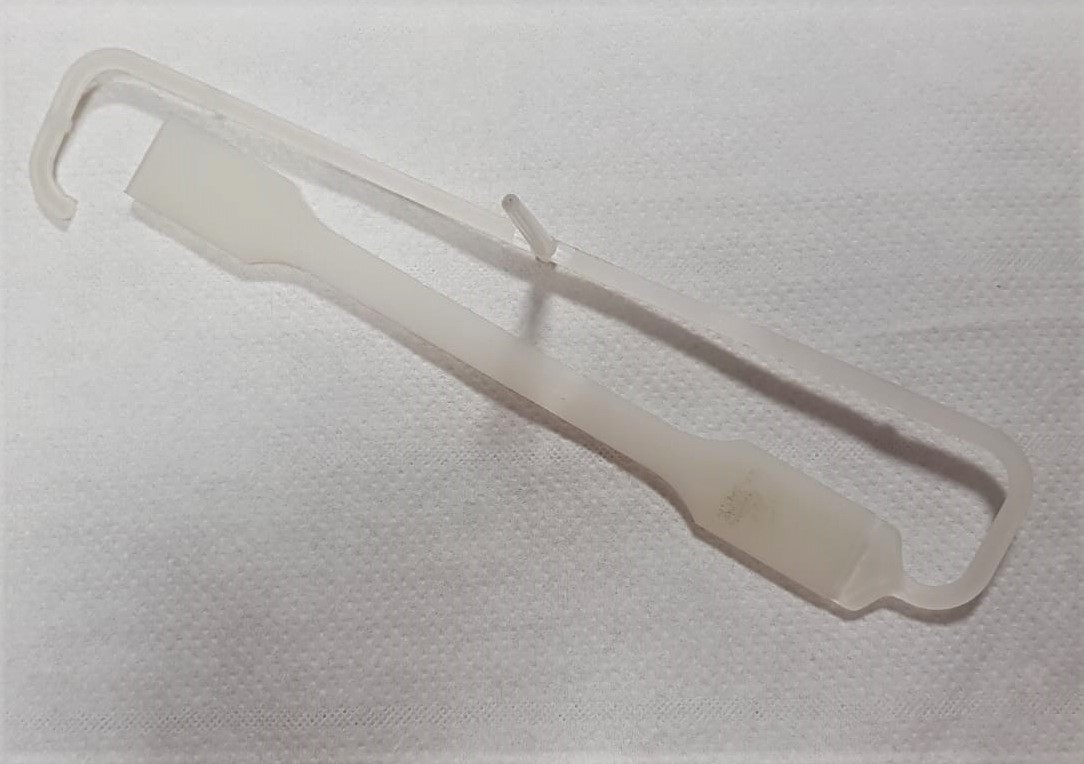
\includegraphics[scale=0.21]{PA11ISO}} \\
\subfloat[][]
{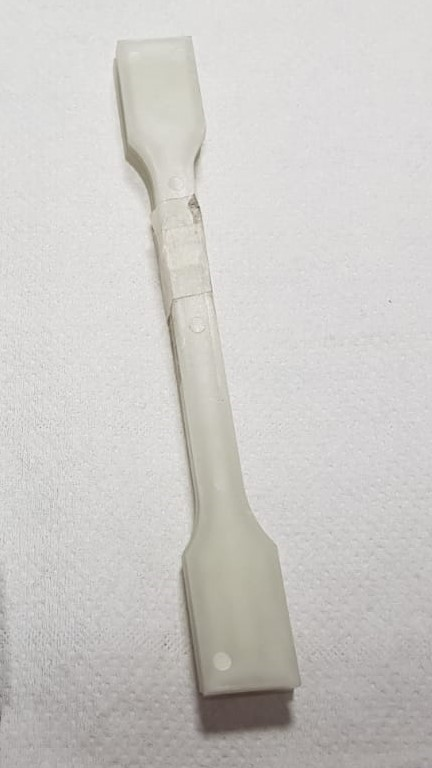
\includegraphics[scale=0.25]{PPW}} \qquad
\subfloat[][]
{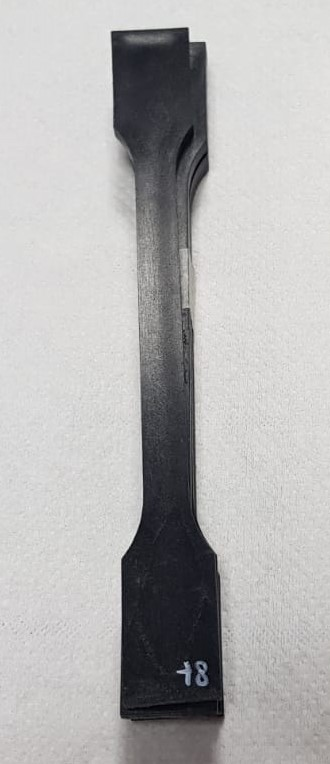
\includegraphics[scale=0.25]{PPB}} \qquad
\subfloat[][]
{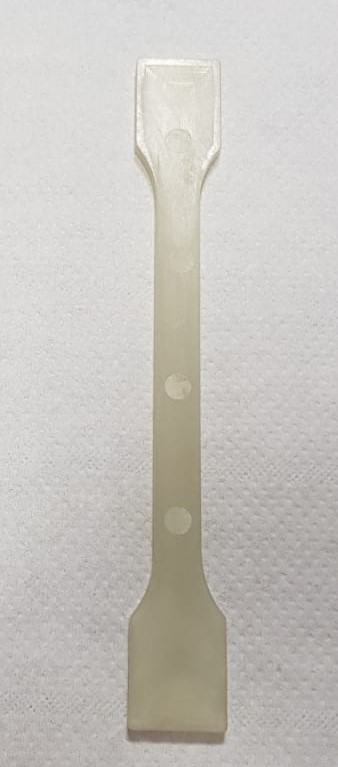
\includegraphics[scale=0.25]{PA6GF}}
\captionsetup{justification=centering}
\caption{ISO samples: a) POM; b) PA11; c) PP-GF30; d) PP-GF35; e) PA6-GF50. }
\label{fig:ISO}
\end{figure}
\newpage
In Table \ref{tab:ISO} different types of ISO speciments are classified with their sizes.

\begin{table}[htp]
\centering
$
\begin{array}{cccl}
\toprule
\textbf{Figure} & \textbf{Material} & \textbf{Size}\,(mm) & \textbf{Description} \\
\midrule
\text{a} & \text{POM} & 9.74 $x$ 3.94 $x$ 167.06 & \text{white and presence of cold junction}\\
\text{b} & \text{PA11} & 9.86 $x$ 4.05 $x$ 168.98 & \text{opaque and white}\\
\text{c} & \text{PP-GF30} & 9.88 $x$ 4.00 $x$ 172.11 & \text{white and stiff}\\
\text{d} & \text{PP-GF35} & 9.80 $x$ 4.00 $x$ 171.86 & \text{black and stiff}\\
\text{e} & \text{PA6-GF50} & 9.99 $x$ 3.98 $x$ 154.71 & \text{very stiff}\\
\bottomrule
\end{array}
$
\caption{ISO speciments and characteristics.}
\label{tab:ISO}
\end{table}

In Table \ref{tab:shISO} the values of the shrinkage of ISO samples are reported.

\begin{table}[htp]
\centering
$
\begin{array}{cccl}
\toprule
\textbf{Samples} & \textbf{Longitudinal shrinkage} & \textbf{Transversal shrinkage} & \textbf{Thickness} \\
\midrule
\text{POM} & 0.0280 & 0.0260 & 0.0150 \\
\text{PA11} & 0.0170 & 0.0140 & -0.0120 \\
\text{PP-GF30} & 0 & 0.0120 & 0  \\
\text{PP-GF35} & 0.0008 & 0.0200 & 0  \\
\bottomrule
\end{array}
$
\caption{Shrinkage of ISO samples.}
\label{tab:shISO}
\end{table}

From Table \ref{tab:shISO} it can be noticed that in reinforced polymers the shrinkage is very small, almost negligible. The presence of glass fibers gives to polymers better dimensional stability during cooling.

ASTM speciments are reported in Figure \ref{fig:ASTM}.

\begin{figure}[htp]
\centering
\subfloat[][]
{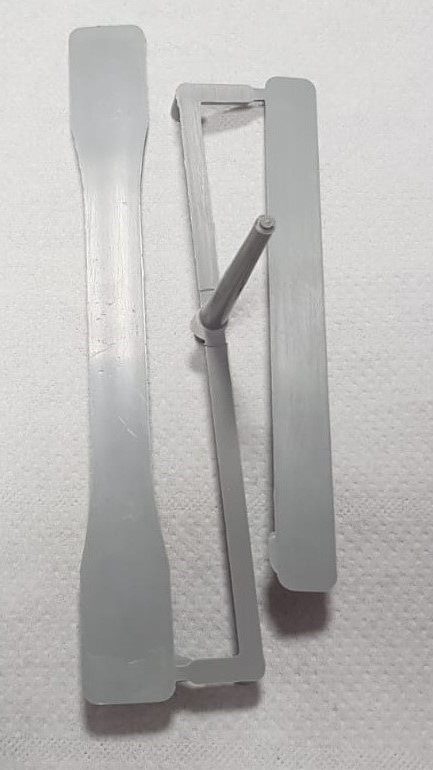
\includegraphics[scale=0.25]{ABS}} \qquad
\subfloat[][]
{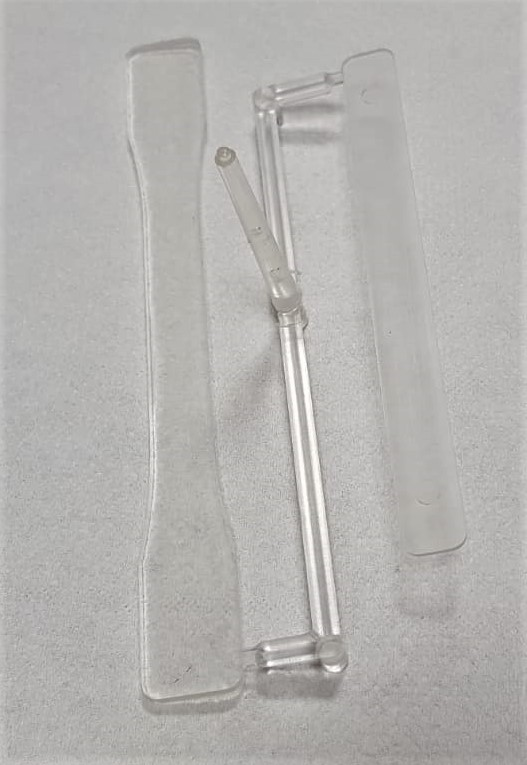
\includegraphics[scale=0.25]{COC}} \qquad
\subfloat[][]
{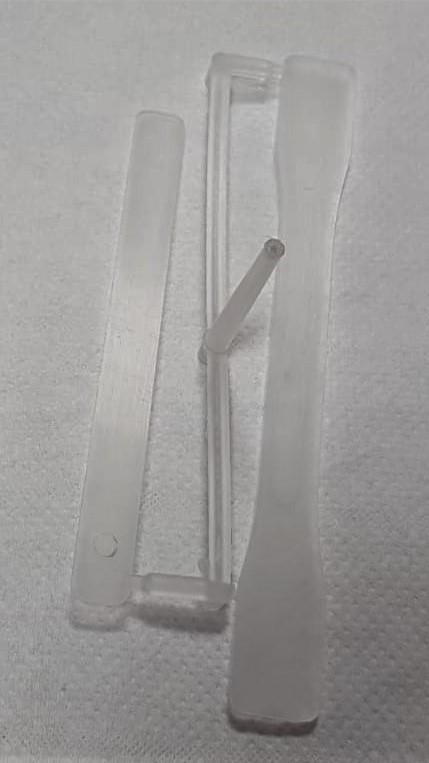
\includegraphics[scale=0.25]{PP}} \\
\subfloat[][]
{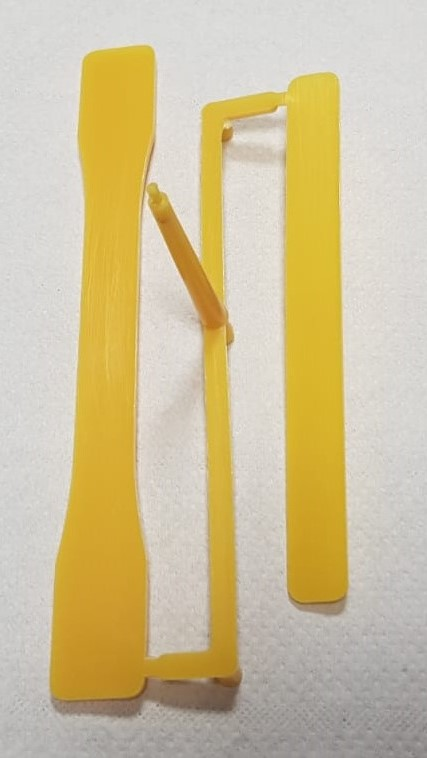
\includegraphics[scale=0.25]{HDPE}} \qquad
\subfloat[][]
{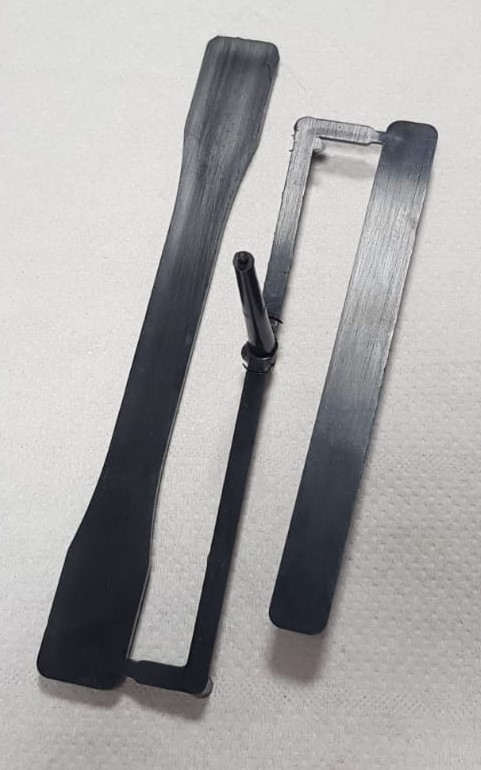
\includegraphics[scale=0.25]{PE-PP}} \qquad
\subfloat[][]
{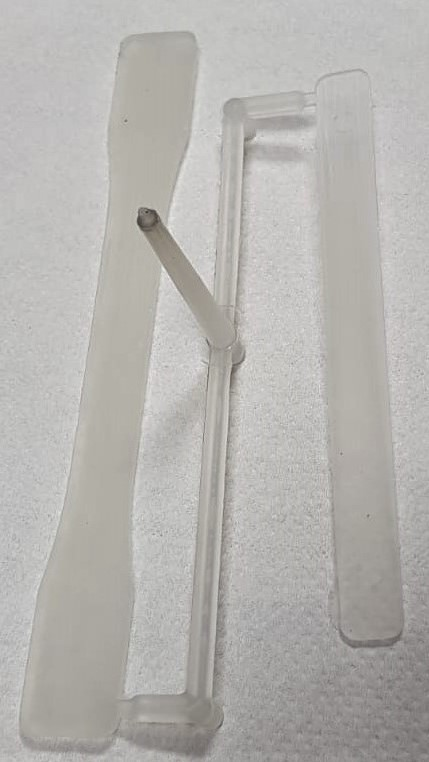
\includegraphics[scale=0.25]{PA11ASTM}} \\
\subfloat[][]
{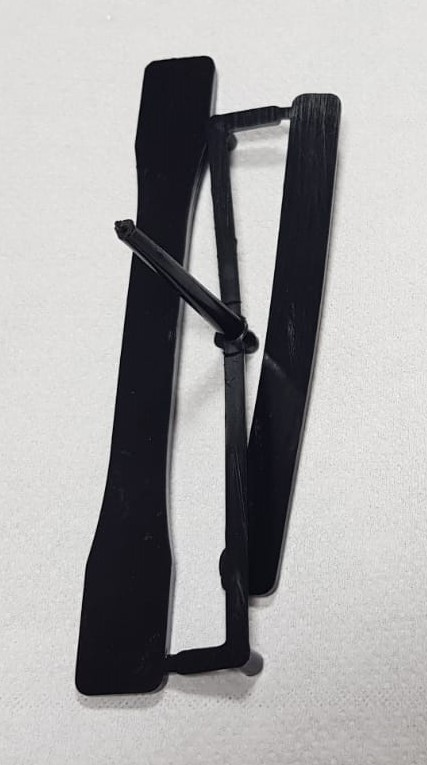
\includegraphics[scale=0.27]{TPU}}
\captionsetup{justification=centering}
\caption{ASTM samples: a) ABS; b) COC; c) PP; d) HDPE; e) PE/PP\ \text{blend}; f) PA11; g) TPU. }
\label{fig:ASTM}
\end{figure}

In Table \ref{tab:ASTM} different types of ASTM speciments are classified with their sizes.
\begin{table}[htp]
\centering
$
\begin{array}{ccccl}
\toprule
\textbf{Figure} & \textbf{Material} & \textbf{Weight}\,(g) & \textbf{Size}\,(mm) & \textbf{Description} \\
\midrule
\text{a} & \text{ABS} & 14.78 & 12.77 $x$ 3.27 $x$ 163.55 & \text{grey and flexible}\\
\text{b} & \text{COC} & 14.07 & 12.64 $x$ 3.30 $x$ 164.04 & \text{transparent and glassy}\\
\text{c} & \text{PP} & 12.28 & 12.6 $x$ 3.35 $x$ 162.29 & \text{opaque and flexible} \\
\text{d} & \text{HDPE} & 12.73 & 12.54  $x$ 3.33 $x$ 160.0 & \text{yellow and very flexible} \\
\text{e} & \text{PE/PP}\ \text{blend} & 13.30 & 12.66 $x$ 3.31 $x$ 161.58 & \text{matt black and flexible} \\
\text{f} & \text{PA11} & 14.00 & 12.6 $x$ 3.35 $x$ 162.29 & \text{very similar to PP} \\
\text{g} & \text{TPU} & 17.16 & & \text{glossy black and most flexible} \\
\bottomrule
\end{array}
$
\caption{ASTM speciments and characteristics.}
\label{tab:ASTM}
\end{table}
\\

In Table \ref{tab:shASTM} the values of the shrinkage of ASTM samples are reported.

\begin{table}[htp]
\centering
$
\begin{array}{cccl}
\toprule
\textbf{Samples} & \textbf{Longitudinal shrinkage} & \textbf{Transversal shrinkage} & \textbf{Thickness} \\
\midrule
\text{ABS} & 0.0088 & -0.0058 & -0.0220  \\
\text{COC} & 0.0303 & 0.0126 & -0.0410 \\
\text{PP} & 0.0164 & 0.0032& -0.0470 \\
\text{HDPE} & 0.0303 & 0.0126 & -0.0410 \\
\text{PE/PP blend} & 0.0207 & 0.0015 & -0.0340 \\
\text{PA11} & 0.0164 & 0.0032& -0.0470 \\
\text{TPU} &  &  & \\
\bottomrule
\end{array}
$
\caption{Shrinkage of ASTM samples.}
\label{tab:shASTM}
\end{table}

From Table \ref{tab:shASTM} it can be observed that semycristalline polymers (such as PP, HDPE, PA11) have higher values of shrinkage respect to amourphous polymers (such ABS and COC).

In Table \ref{tab:pesi} weights and densities of ASTM samples are reported. Densities have been taken from .....

\begin{table}[htp]
\centering
$
\begin{array}{ccc}
\toprule
\textbf{Samples} & \textbf{Weight}\,(g) & \textbf{Density}\,(g/cm^3) \\
\midrule
\text{ABS} & 14.78 & 1.04-1.12  \\
\text{COC} & 14.07 & 1.02 \\
\text{PP} & 12.28 & 0.85-0.94 \\
\text{HDPE} & 12.73 & 0.93-0.97 \\
\text{PE/PP blend} & 13.3 & 0.86-0.95 \\
\text{PA11} & 14.00 & 1.04 \\
\text{TPU} & 17.16 & 1.23-1.35 \\
\bottomrule
\end{array}
$
\caption{Weight and density of ASTM samples.}
\label{tab:pesi}
\end{table}

For PE/PP blend it has been considered a blend constituted by PE/PP $50\%$. From Table \ref{tab:pesi} it can be noticed that, for the same volume, weights of samples are in accordance with values of densities taken from literature. 


\end{document}